To compare different codes and decoding schemes
we introduce the concept of thresholds, whereby the threshold
of a specific code of scalable distance with a specific decoding 
scheme is defined as the physical error rate $per$ at which the logical
error rate becomes greater than $50\%$ in the limit of infinite 
distance. \\
Thresholds can vary depending on the error model, i.e. 
some codes can have a higher threshold for X than for Z errors.
For simplicity's sake in the following, we will assume equal 
X, Y and Z error rates of $\frac{per}{3}$.

\begin{figure}[h!]
    \centering
    \subfigure[Surface code MWPM thresholding overview]{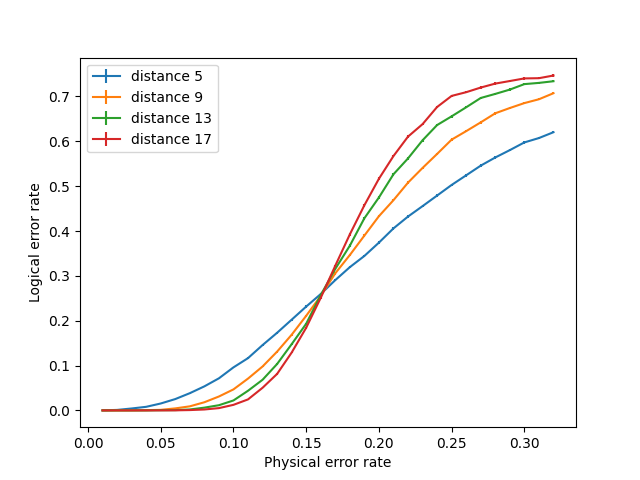
\includegraphics[width=0.4\textwidth]{img/figures/thresholds/surfaceThresholdOverview.png}}\hfill
    \subfigure[Detailed view for precise threshold determination]{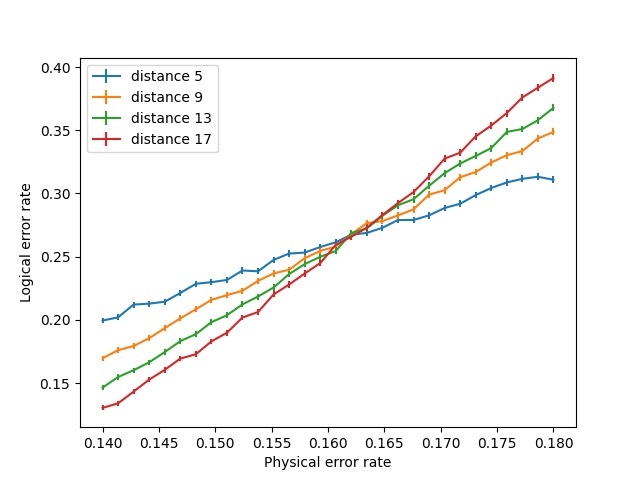
\includegraphics[width=0.4\textwidth]{img/figures/thresholds/surfaceThresholdVeryPrecise.png}}
    \caption{Thresholding of the surface code using the MWPM decoder implemented in the PyMatching \cite{MWPMDecoder} library.
    Generating code can be found in Appendix \ref{App: surface_thresholding}}
    \label{fig:surface_threshold}
  \end{figure}

Using this error model, we found a threshold of $16.3\pm 0.5 \%$ from
figure \ref{fig:surface_threshold} and $16.0\pm 0.5\%$ from figure
\ref{fig:toric_threshold} for the surface and toric code respectively. 
Their thresholds are within single error margins of each other, and 
can therefore be called identical.

\begin{figure}[h!]
    \centering
    \subfigure[Toric code MWPM thresholding overview]{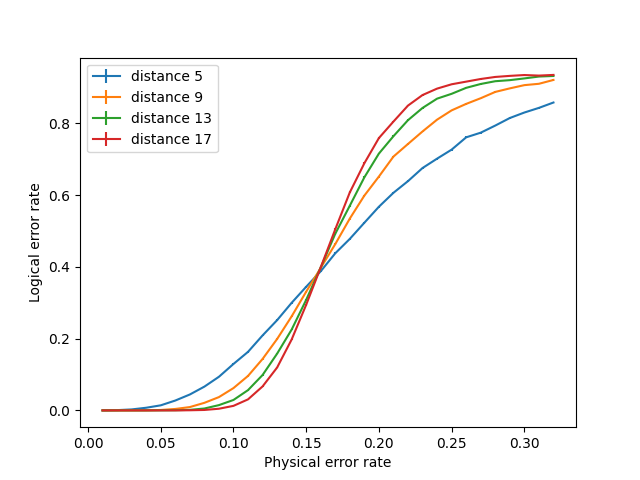
\includegraphics[width=0.4\textwidth]{img/figures/thresholds/toricThresholdOverview.png}}\hfill
    \subfigure[Detailed view for precise threshold determination]{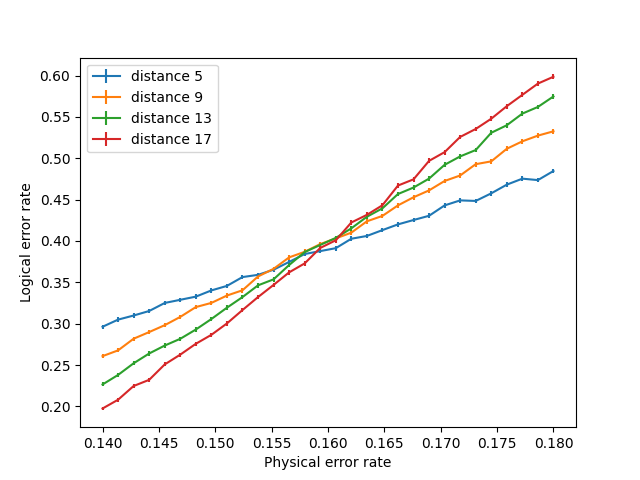
\includegraphics[width=0.4\textwidth]{img/figures/thresholds/toricThresholdVeryPrecise.png}}
    \caption{Thresholding of the Toric code using the MWPM decoder implemented in the PyMatching \cite{MWPMDecoder} library.
    Generating code can be found in Appendix \ref{App: surface_thresholding}}
    \label{fig:toric_threshold}
\end{figure}
\newpage
Since the Steane code for which we generated a lookup table is not 
a distance-scalable code, only a $pseudo$-threshold can
be found here, i.e. the crossing point to worse performance than unencoded
information. As can be seen in figure \ref{fig: steane_threshold}, the
pseudo-threshold is somehow very bad. I do not know why.

\begin{figure}[h!]
	\begin{center}
	\captionsetup{justification=centering,margin=2cm}
	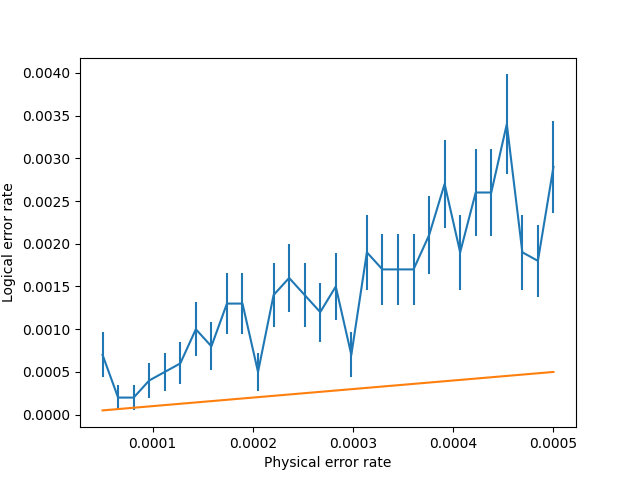
\includegraphics[scale=0.4]{./img/figures/thresholds/steaneLookupThreshold.png}\\
	\caption{Lookup table pseudo threshold for the Steane code, generating code can be found in Appendix
    \ref{App: steane_thresholding}}
        
	\label{fig: steane_threshold}
	\end{center}
\end{figure}

\newpage

On the color code, we found a threshold of $<0.0001\%$ using the 
lookup table decoder on the Steane code and could not find a threshold
for the scalable hexagonal toric color code, as our code does not work there yet.

% $c\pm b\%$ using the 
% lifting decoder for the scalable hexagonal toric color code. 
% (Reference appendix code, include a figure)
\newpage